\section{Motivation}

The effects of climate change increase in severity every year. From 1980 to present, the global temperature anomaly --- defined as the difference between the current average global temperature and the average temperature from 1951 to 1980 --- has steadily increased to 1.02 $^{\circ}$C.  One factor contributing to this global climate change is the use of fossil fuels.  In relatively recent years, there has been a growing push for energy technologies that do not rely on fossil fuels, such as nuclear power.  While nuclear technology is currently in use across the world, many of these reactors are older, and facing closure as their licenses run out.  As licenses run out and nuclear power plants are forced to close when there is no replacement reactor, energy companies may be forced to return to fossil fuels to supply the baseline power that nuclear once did.  In addition, most of the current global fleet consists of Gen III reactors, which do not feature the passive safety features and advanced designs of Gen IV reactors.  There is an international effort to support the development of these reactors, led by the \acrfull{gif}.  \acrshort{gif} identified eight goals the design of Gen IV reactors should fulfill, encompassing improvements to sustainability, economics, safety, and non-proliferation \cite{noauthor_home_nodate-1}.

One such class of Gen IV reactor, the high temperature gas-cooled reactor (HTGR), can have a variety of fuel forms. This work concerns itself with pebble-bed \acrshort{htgr}.  Pebble-type fuels consist of a sphere of graphite, approximately the size of a billiard ball, embedded with tri-structural isotropic (TRISO) particles.  TRISO-based fuels are popular in Gen IV reactor design because they are a robust fuel form --- not prone to cracking and stable to higher temperatures than standard \acrfull{lwr} fuel.  This is advantageous to long-term spent fuel safety (though it does make reprocessing much more difficult).  Pebble-type fuels in particular can be refueled online, which reduces the need for planned shutdowns.  However, HTGRs are typically very large designs, which can be prohibitively costly, or simply unneeded in some use cases.

To avoid this size restriction, another class of reactor was designed - the \acrfull{smr}.  These reactors are smaller than the conventional \acrshort{lwr} seen in the USA today.  \acrshort{smr}s are often small enough to be shipped in a standard shipping truck or train.  Owing to their small size, they are also easier and cheaper to manufacture.  One can deploy an SMR in a variety of new settings, such as isolated towns or work sites, or station many together in one location to fill the role of a single larger reactor.  But there exists a class of reactor even smaller than the \acrshort{smr} --- the microreactor.  Microreactors generally have a capacity of 70 MWth or less and are often deployed in areas only needing a small amount of power, used for research and testing, or used to supply heat for other industrial processes, such as producing hydrogen.  Down-sized reactors, such as SMRs or microreactors, have a few inherent safety benefits over their larger cousins, prompting their development.  The smaller scale of the reactor pressure vessel (RPV) makes the large active cooling loops of contemporary commercial nuclear reactors unneccesary.  For smaller reactors, passive systems relying on natural convection and surface heat transfer remove decay heat after something such as a station black-out (SBO).  Under normal operation with station power, supplementary fans and surface coolers can aid heat removal \cite{reutler_advantages_1984}.


This work modeled a 200MWth pebble-bed high-temperature gas-cooled \acrshort{smr} based on existing designs.  We call this 200MWth reactor the Sangamon200.  Sangamon200 is meant to reflect a "classic" Gen IV reactor design.  A smaller 20MWth design was created by scaling down the Sangamon200 model.  The 20MWth model, hereafter referred to as Sangamon20, is a generic design for use in testing and analysis.  This model is simplified to provide a foundation for investigating core neutronics and fuel isotopics without additional features beyond the randomness and heterogeneity of the pebbles inside, which is the focus of this study.


\section{Objectives}

This work briefly describes a 200 MWth pebble-bed HTGR SMR, inspired by concepts from the PBMR \cite{venter_pbmr_2005}, \cite{noauthor_pebble_2017} and X-Energy \cite{harlan_x-energy_2018} reactors, henceforth named Sangamon200.  This work established the larger reactor as a baseline for the scaled-down 20 MWth model, Sangamon20 that is the focus of this work.

However, any full-core pebble-bed reactor model will have significant computational load.  In order to make running such models less demanding, it is sometimes necessary to make simplifications that are not reflected in a real-world core.  A pebble-bed reactor already has multiple layers of heterogeneity - the locations of the TRISO particles in the pebbles are randomly generated as well as the location of the fuel pebbles in the core.  Pebble location aside, there are seven fuel compositions also distributed uniformly and randomly throughout the core.  Previous work, in contrast, often used a lattice arrangement to set pebble locations. As said before, Sangamon20 uses random pebble dispersal.  This means that there are a theoretically infinite number of Sangamon20 designs that \emph{could} exist, with only pebble location changing.  This randomness presents a design and licensing challenge --- even if one can demonstrate a particular permutation of a given pebble bed reactor is safe, is that model sufficient to prove all variations are?  To help answer this question, the shuffling test was performed (see: Methods) to provide a few variations to compare with the "control" model. Another source of variation in the model is using a symmetry assumption.  When a symmetry condition is used, Serpent takes a user-defined fraction of the core (for this thesis, $\frac{1}{6}$) and uses it to represent the entire core.  Assuming a symmetry condition may make the core easier to model, but it also introduces error.  One can imagine that if this user-defined region happens to have a higher fraction of a particular burnup of pebbles than the rest of the reactor, the results wouldn't accurately reflect the whole-core.  To investigate the a series of simulations running the Sangamon20 model while utilizing a radial symmetry condition were analyzed (henceforth called the symmetry test, see section \autoref{meth-sens}, Table \ref{table:sens}).  This not only shows the impact on this specific design, but also provides insight on the effects such a simplification may have on a more intricate model (where simplification may become a necessity).

\section{Background}
\label{sec:intro-background}

While HTGRs and pebble bed reactors have had a recent resurgence in interest and research, they are, in fact, an older concept.  The following subsections describe early \acrshort{htgr} concepts, reactors, and how they contributed to our present knowledge of \acrshort{htgr}s.  Even though experimental data collection and analysis is not the goal nor focus of this thesis, the previous empirical data and experience informs modern-day HTGR design and modeling.  Addtionally, as there have not been many modern-day HTGR designs that have come to fruition --- many have been terminated in one form or another before they were built --- these early experimental and commercial reactors provide us with valuable insight that may otherwise be inaccessible.

\subsection{The High Temperature Gas Cooled Reactor: Beginnings and Concepts}

\acrshort{htgr}s are a prominent Generation IV reactor design which often uses helium as a coolant, and graphite as a moderator.  Their fuel form uses TRISO particles, which consist of a small kernel of fuel, less than half a millimeter across, surrounded by layers of carbon and silicon carbide to protect the fuel kernel and prevent the leakage of radioisotopes.  Fuel elements are made by embedding these TRISO particles in graphite.  In prismatic HTGRs, the graphite is in the shape of hexagonal columns.  In pebble-bed reactors, the graphite is in the shape of six cm diameter spheres.  Many of these pebbles enter the core through the top, and slowly move down in a manner similar to grain in silos.

Preliminary concepts for a gas-cooled reactor existed as early as 1942.  Farrington Daniels is attributed with establishing the first theoretical designs.  Professor Daniel's work with Oak Ridge National Laboratory (ORNL) nailed-down the most basic characteristics of the HTGR.  The choice of helium for coolant, graphite for moderator, the direct gas turbine cycle, and the use of uranium or thorium carbides for fuel all came from his work \cite{simnad_early_1991}.

\begin{figure}[h!]
\centering
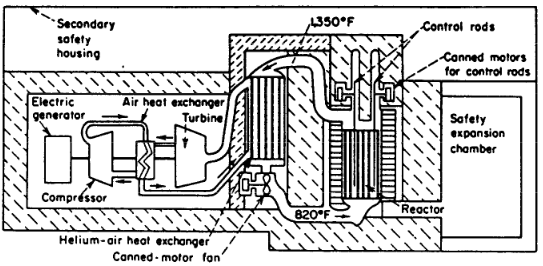
\includegraphics[width=0.6\linewidth]{figures/daniels-1}
\caption{Side-View of the 1955 Daniels' Concept, \cite{simnad_early_1991}}
\label{fig:daniels-1}
\end{figure}
\begin{figure}[h!]
\centering
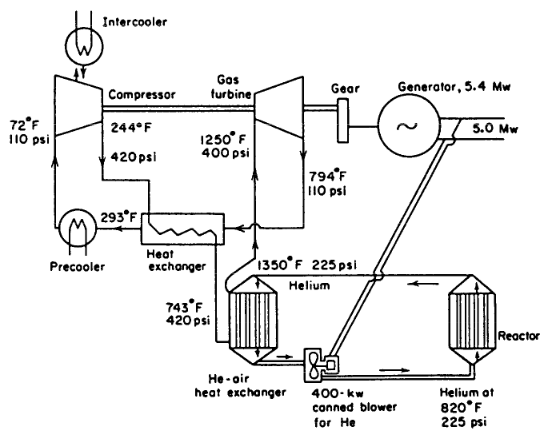
\includegraphics[width=0.6\linewidth]{figures/daniels-2}
\caption{Diagram of Coolant Flow in the 1955 Daniel's Concept, \cite{simnad_early_1991}}
\label{fig:daniels-2}
\end{figure}

Figures \ref{fig:daniels-1} and \ref{fig:daniels-2} show the 1955 concept in the design by Daniels et al.  A key difference between the Farrington Daniels et al designs and modern HTGRs is the fuel form.  While modern designs use TRISO particles embedded in graphite, the Daniels et al design used solid graphite blocks, with channels for both coolant and fuel.  Within the fuel channels, fuel loaded in either a pellet or cartridge form, both a mixture of 10$\%$ uranium dicarbide and graphite powder.  In addition to these fuel channels, the design included an outer ring of graphite reflector in which used thorium to breed $^{233}U$.  Control rods were of a boron-containing molybdenum.  Steel wires that would melt in the case of an accident held more of the same above the core, and would drop the safety rods in case of an accident \cite{simnad_early_1991}.

\subsection{Earliest Operational HTGRs}

The earliest operational HTGRs came online in the 1960s.  These early reactors are discussed in the sections below: Dragon, operating in the UK; Peach Bottom 1, in the US; and the AVR, from Germany.  Of these three, only Peach Bottom 1 was a commercial-scale demonstration - the others, Dragon and the AVR, were experimental reactors.  Of particular interest is the AVR which is the only pebble-bed reactor of the three.  Experiments in the AVR not only provided empirical data on the inner-core temperatures inside the AVR core, but also tested accident response, and observed a "pebble dust" that accumulated in the AVR over its operation --- including its activity.

\subsubsection{Dragon}
\label{dragon}

The Dragon prismatic HTGR was a test reactor operated in Winfrith, UK, by the Organization for Economic Co-operation and Development from 1964 to 1975, making it the oldest of the reactors discussed in this chapter.  It operated with inlet and outlet temperatures of 350 \textdegree C and 750 \textdegree C, respectively, and at 20MWt \cite{beck_high_nodate}.  Dragon's main purpose was to test reactor materials, with an emphasis on fuels.  It originally used uranium and thorium as fuel but switched to a purely uranium-based fuel with a lower enrichment later in life.  The fuel elements themselves were similar in shape to the Daniels et al design: hexagonal prisms with fuel rod channels.

Contrary to the fuel philosophy seen today, Dragon originally allowed fission products released from fuel elements into the circulating helium coolant.  The fission products are then purged from the helium.  However, Dragon later switched to a coated-particle fuel when it became clear that having such fission product releases were difficult to manage \cite{simnad_early_1991}.

\subsubsection{Peach Bottom 1}\
\label{peach}

Peach Bottom 1 operated from 1966 to 1974, by the Philadelphia Electric Company and was located in Delta, Pennsylvania \cite{beck_high_nodate},\cite{noauthor_peach_nodate}.  It was the first operational HTGR in the US, and the first to produce electric power.  It was slightly larger than Dragon, at a nameplate capacity of 115 MWt/40MWe and a slightly lower operating temperature range at 327\textdegree  C to 700\textdegree  C inlet to outlet \cite{beck_high_nodate}.  Like Dragon, Peach Bottom 1 was a prismatic reactor; however, Peach Bottom used coated uranium and thorium carbide particles coated by a single layer of pyrolytic carbon.  However, after multiple fuel failures, Peach Bottom upgraded to bistructural isotropic, or BISO, fuels by adding an additional layer of pyrolytic carbon.  Peach Bottom would later upgrade the fuel once again by adding a silicon carbide layer, forming TRISO particles \cite{beck_high_nodate}.  One operational benefit of upgrading to TRISO particles from BISO particles was that the superior fission product retention meant that Peach Bottom 1 could remove the helium purging systems.  In addition to the inner fuel region, Peach Bottom, like the Daniels et al design, bred $^{233}U$ in an outer region using thorium.

Beyond changing the number and materials for fuel coatings, the experiences in Peach Bottom 1 helped to develop HTGR fuel elements.  Operators saw that they could dilute the fuel with graphite moderating material more so than other diluents.  This has the advantage of saving fuel material, improving heat transfer, and reducing radiation damage.  Additionally, operational experience showed that, in order to prevent the creation and buildup of $^{236}U$ and $^{237}Np$, which are neutron poisons, the $^{235}U$ and $^{233}U$ should be kept separate \cite{simnad_early_1991}.  In the end, however; Peach Bottom 1 closed after the Philadelphia Electric Company determined its size made it no longer economically viable.

\subsubsection{AVR}
\label{avr}

The Arbeitsgemeinschaft Versuchsreaktor (AVR) was an experimental pebble-bed reactor operated in and by the Jülich Research Center (in Jülich, Germany) from 1967 to 1988.  It had a capacity of 46 MWt/15MWe, with inlet and outlet temperatures of 275\textdegree  C and 950\textdegree  C \cite{beck_high_nodate}.  The AVR used a combination of uranium and thorium fuels, though it began with bi-structural isotropic (BISO) particles.  The core held around 100,000 graphite pebbles, only a third of which had fuel in them.

Despite not being built for experimental purposes, the AVR still housed many experiments that improved our body of knowledge on HTGR technology.  During the first few years of its life, the goal of the AVR was to demonstrate that it was a reliable technology --- that the reactor could operate safely, that they could control the core power and temperatures, safely shutdown, and remain sub-critical for long periods of time.  After this inital period, the AVR shifted focus to allow various experiments including: observing core temperature distributions, accident analysis, and fuel testing.  The AVR also shifted from highly enriched to low enriched fuel over time, which caused a variation in fuel pebble compositions, on top of the range of compositions inherent to a multi-pass pebble cycle due to varying burnup.

The AVR also provided data to validate simulations of pebble-bed reactors, and conducted an experiment to better characterize the radial distribution of temperatures in the core \cite{noauthor_results_1990}.  Operators loaded a number of marked pebbles into the core, each housing a series of wires that would melt at a certain temperature, the lowest being 655\textdegree  C, the highest 1280\textdegree  C.  Those conducting the test tracked pebble location using flow data, and examined them after they were ejected to determine what temperatures the pebbles experienced.  Despite the outlet temperature being 950\textdegree  C, multiple pebbles experienced a temperature greater than or equal to the 1280\textdegree C maximum temperature in the melt wires.  The results noted that these pebbles went through a zone with a spike in local power density, which could account for the temperature spike \cite{noauthor_results_1990}.

The AVR also demonstrated the inherent safety of HTGR reactors in accident scenarios by purposefully causing failures of the active cooling system.  In the first, the coolant blowers were shutoff, and no shutdown rods inserted, while operating at full power.  The operators additionally shut the main circuit valves to prevent natural circulation to regions outside the active core.  Overall, the changes to core temperatures were unremarkable.  The hottest regions cooled, while the coldest regions warmed up.  Additionally, due to negative temperature feedback coefficients, the reactor power immediately declined in response to the transient event.  The temperature slowly rose to 2 MW again over 24 hours, leveling out around 300 kW.  A further test provided data on loss of coolant and depressurization accidents.  As before, the core temperature changes were unremarkable.  The upper core region cooled, while the lower, originally cooler core region slowly rose in temperature.  The experiment's thermal data helped validate HTGR computer models by providing a real-world benchmark.  This meant that the results to aid in the analysis of other HTGRs \cite{noauthor_results_1990}.

Beyond accident safety, the AVR allowed for testing and demonstration of the safety qualities of TRISO and BISO fuel elements; especially relating to high temperature tolerance, and fission product retention.  Initial tests used BISO based pebbles, then later transitioned to TRISO, then to low-enriched-uranium (LEU) TRISO pebbles.  The TRISO-LEU pebbles had good fission product retention compared with their BISO-based predecessors, based on the the activity of samples taken from the circulating helium.  Beyond radioisotopes being directly released into the coolant gas, the AVR also showed that in order to accurately characterize the source term of am HTGR pebble bed reactor, one must take the dust from the pebbles into account.  Dust from the pebbles bumping and scraping against each other deposited on reactor surfaces in the primary loop.  Sixty kg of dust had accumulated by the end of the reactor's life, which averages to 3 kg of dust each year.  Measurements of specific activity in the dust showed that the activities of $^{137}Cs$, $^{134}Cs$, $^{131}I$, $^{90}Sr$, and $^{60}Co$ were on the order of $\frac{Bq}{g}$ (see Table \ref{table:gas-acc} and Table \ref{table:dust-acc}).  Even though relatively little dust accumulates, the activity of this dust is fairly high, especially compared to the activity of the coolant gas \cite{noauthor_results_1990}.  This dust can become mobile in an accident scenario, potentially being released into the environment, or inhaled.

\begin{table}[h!]
\centering
\caption{Helium Coolant Specific Activities in the AVR, reproduced from Table 2 in \cite{gottaut_results_1990} --- Results of experiments at the AVR Reactor by H.Gottaut and K.Krüger}
\begin{tabular}{ c   c }
\hline
Isotope & Specific Activity in Primary Coolant Gas $[\frac{Bq}{m^3}]$  \\
\hline
$\sum$ Fission noble gas & $4.6\times10^{08}$  \\
$^{3}H$ & $3.7\times10^{07}$  \\
$^{14}C$ & $1.9\times10^{07}$  \\
$^{137}Cs$ & $3.0\times10^{02}$ \\
$^{131}I$ & $5.2\times10^{02}$ \\
$^{110m}Ag$ & $4.9\times10^{01}$  \\
$^{90}Sr$ & $2.0\times10^{02}$  \\
$^{60}Co$ & $1.0\times10^{01}$ \\
\hline
\end{tabular}
\label{table:gas-acc}
\end{table}
\begin{table}[h!]
\centering
\caption{Pebble Dust Specific Activities, reproduced from Table 3 in \cite{noauthor_results_1990} --- Results of experiments at the AVR Reactor by H.Gottaut and K.Krüger}
\begin{tabular}{ c   c }
\hline
Isotope & Specific Activity in Dust $[\frac{Bq}{g}]$  \\
\hline
$^{137}Cs$ & 2 - 96  \\
$^{134}Cs$ & 0.7 - 27 \\
$^{131}I$ & 0 - 3  \\
$^{110m}Ag$ & 0.1 - 43 \\
$^{89}Sr$ & 0.6 - 42 \\
$^{90}Sr$ & 19 - 363  \\
$^{60}Co$ & 0.2 - 8 \\
\hline
\end{tabular}
\label{table:dust-acc}
\end{table}

\subsection{Earliest HTGRs: Conclusion}

The three earliest operational HTGRs have been discussed in Sections \autoref{dragon}, \autoref{peach}, and \autoref{avr}.  Even though Dragon and Peach Bottom 1 are not pebble-bed reactors, they still used TRISO particle fuels, and still provided experience in HTGR operation and management.  The AVR, meanwhile, was a pebble-bed reactor, and not only provided general HTGR experience, but also provided pebble-fuel specific data, such as on pebble dust accumulation and activity.  The experience from these reactors helped to inform the design of modern HTGRs, especially in regards to providing experimental data to validate computational models against.